\section{Problemática}
En el proceso actual de la División de Innovación Academica de la Dirección de Educación Superior(DES), se identifico como área de oportunidad la elaboración y revisión de Programas de Estudio de las Unidades de Aprendizaje para la creación o rediseño de un Plan de Estudios. Debido a las siguientes situaciones:\\
\begin{itemize}
    \item Tiempo desperdiciado en la revisión de detalles innecesarios o información repetida, por ejemplo revisar que concuerden los creditos, las horas, los nombre de las Unidades de Aprendizaje, etc.
    \item Modificaciones a secciones ya aceptadas previamente, es decir que no necesitaban corregirse.
    \item Medio de comunicación externo.
    \item Estructura incorrecta del documento final, por ejemplo saltos de paginas incorrectos, tablas partidas, etc.
    \item Correcciones ignoradas.
    \item Revisiones incompletas o inexistentes por parte de las Unidades Académicas.
\end{itemize}
\begin{figure}[H]
	\centering
	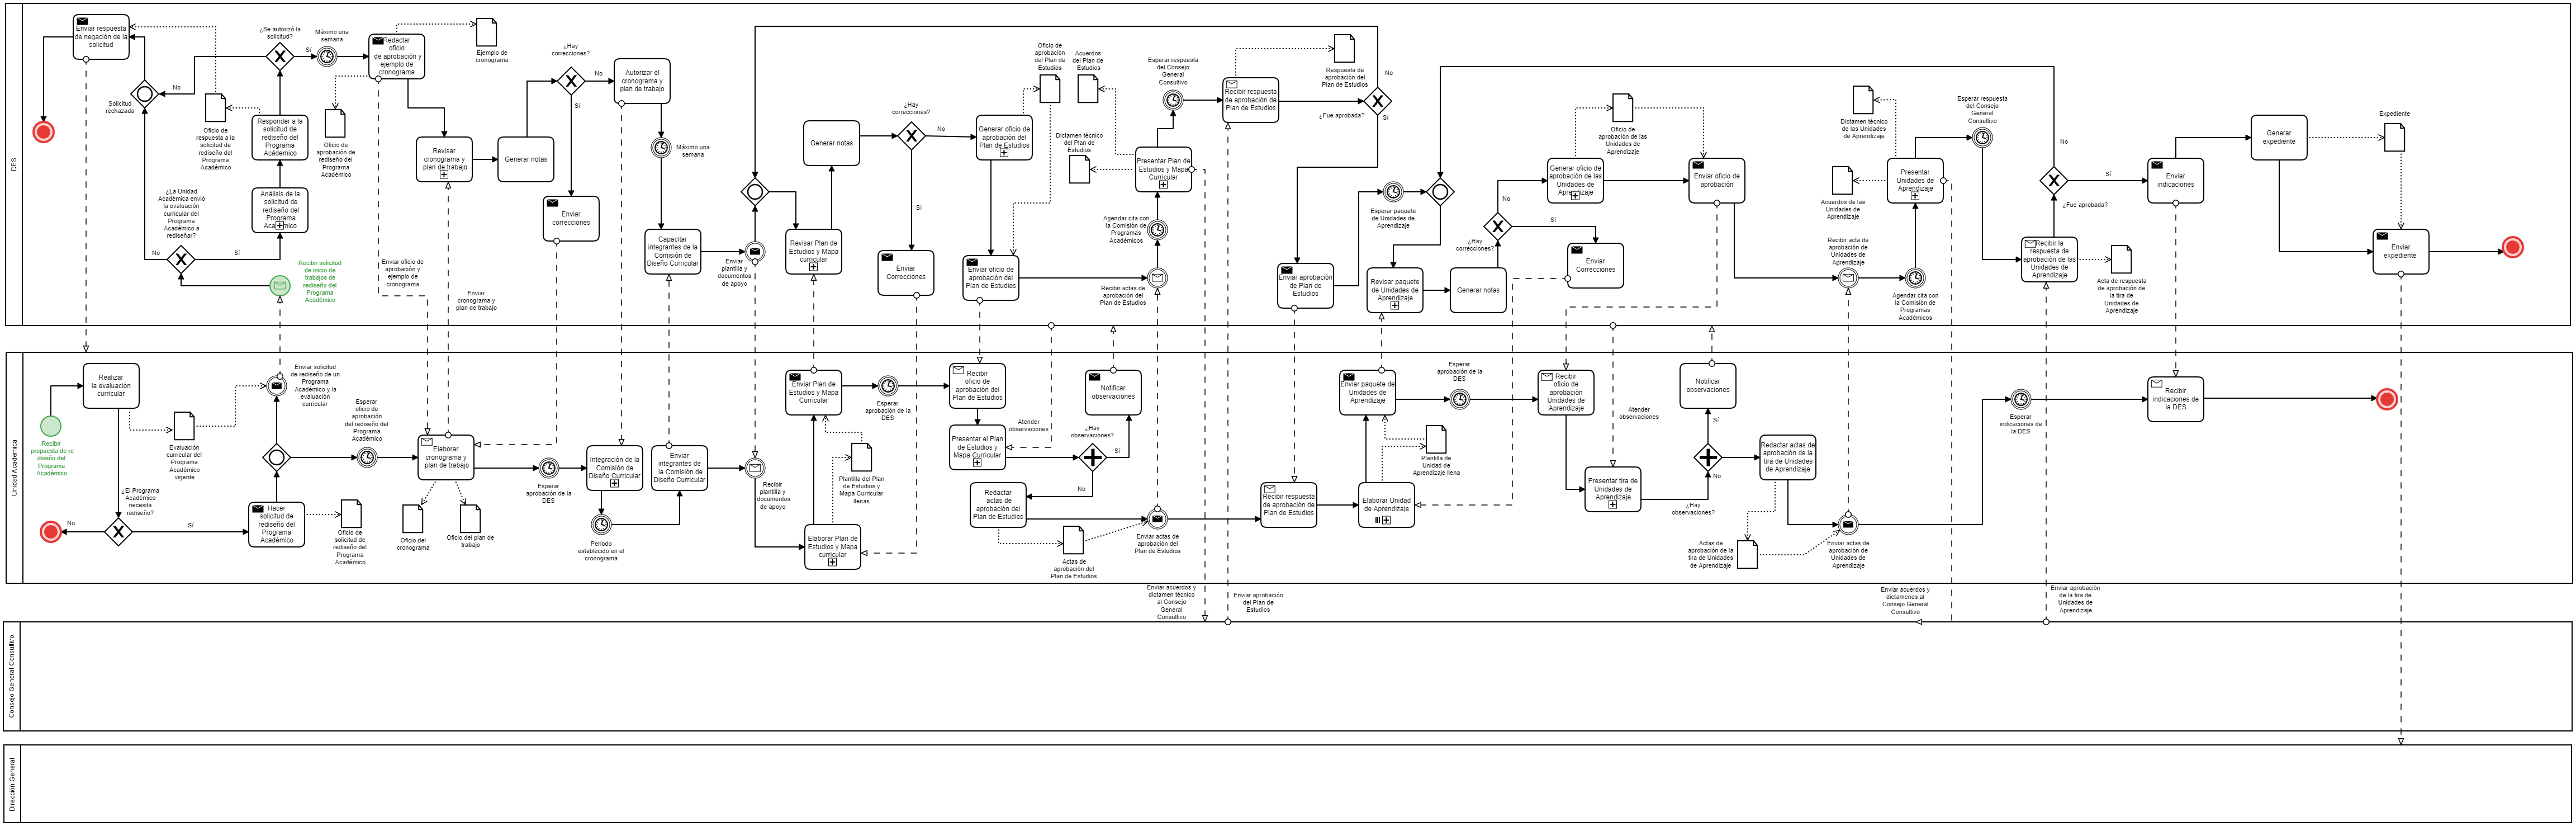
\includegraphics[width=0.9\linewidth]{images/Procesos/MacroProceso}
	\caption{Modelado del Negocio}
\end{figure}
